
%----------------------------------------------------------------------------------------
 %	CHAPTER 6
 %----------------------------------------------------------------------------------------
 \chapterimage{ch6.pdf} % Chapter heading image
 \chapter{Software tool}
In this chapter we explain the software toolkit provided in this course for empirical error analysis. The tool may be used to:
\begin{itemize}
 \item obtain visualizations of point-sets generated by a sampling pattern (sec.~\ref{sec:ptanalyzer});
 \item visualize Fourier spectra (sec.~\ref{sec:Fanalyzer}); 
 \item compare errors across Monte Carlo estimators that use different sampling strategies (sec.~\ref{sec:erranalyzer}); 
\end{itemize}
Sampling is performed on 2D domains only (unit square) and therfore integrands are 2D as well. 

\section{The C++ tool}
\subsection{Set up (Ubuntu)}
The source code may be downloaded from the git repository \url{git:} \KARTIC{put repo here}. Before building the tool the following need
to be installed: cmake, CGAL, ZLIB. On Ubuntu, they may be installed using apt-get. 
\begin{tcolorbox}
 sudo apt-get install cmake \\
 sudo apt-get install libcgal-dev \\
 sudo apt-get install zlib1g-dev 
\end{tcolorbox}
 To build the tool first create a build subdirectory; then run cmake and make within the build directory. The bash commands are shown below. 
\begin{tcolorbox}
  git clone --recursive  git:// \\
  cd NAME OF REPO\\
  mkdir build\\
  cd build\\
  cmake ../ \\
  make\\
  cd ..
\end{tcolorbox}
The binary for empirical error analysis, `eea', is located in the build directory. The `--recursive' argument automatically clones submodules that are dependencies of the toolkit. Currently the dependencies are: \KARTIC{List dependencies.} Executing the binary without any arguments will display a list of options that need to be specified. The command line arguments for eea are divided into four sections in the following order:
 %
\begin{tcolorbox}
 ./build/eea -S  ... <-I ...> -A ... -G ...
\tcblower
Here, \\
-S precedes the type of samples to be used and associated parameters. \\
-I precedes the integrand type and its associated parameters \\
-A precedes analyzer name along with associated parameters \\
-G is a general section.~e.~g.~to specify output filenames.
\end{tcolorbox}
 We will refer to these blocks of the command line as sampling, integrand, analysis and general sections. The integrand section is only needed for some types of analyzers.
 
\subsection{Sampling section}
The switch `--stype' is used to specify the type of sampling. Valid options for 'stype' are Random, Jittered, Grid, GJittered, BJittered and correspond to random sampling, jittered sampling, sampling using the regular grid, Gaussian jitter and box jittered sampling respectively. GJittered and Bjittered have associated parameters (width of the Gaussian and size of the box respectively) which may be specified using appropriate switches. The full list of currently implemented sampler sections is:
\begin{tcolorbox}
  -S --stype Random \\
  -S --stype Jittered \\
  -S --stype Grid \\
  -S --stype GJittered --sigma 0.1 \\
  -S --stype BJittered --boxwidth 0.2 
\tcblower
   --sigma 0.1: Gaussian has a std.dev. that is 0.1 times resolution of the sampling grid \\
   --boxwidth 0.2: uniform jitter but with width 0.2 times that of standard jittered sampling 
\end{tcolorbox}
GJittered and BJittered result in biased estimators. They tend towards unbiased as sigma approaches infinity and boxwidth approaches unity respectively. In addition to the above samplers, stubs have been provided for Poisson disk, Halton, Latin hypercube and Sobol sampling but the core sampling routines are not implemented. 

\subsection{Integrand section}
When an integrand is required for analysis, the switch `--itype' is used to specify the type of integrand. Valid options for `itype' are QuadPix, PWConstant, Gaussian, Disk and Pbrt. They correspond to integrating a binary quad within a square pixel, piecewise constant function within the unit square, a Gaussian, a disk and regions of an image rendered using PBRT~\cite{Pharr:2010:PBR:1854996}. The full list of options is
\begin{tcolorbox}
  -I --itype QuadPix --points 0.1 0.2 0.4 0.3 \\
  -I --itype QuadPix --random \\
  -I --itype PWConstant --npts 10 \\
  -I --itype Gaussian --center 0.3 0.4 --sigma 0.05 0.1 \\
  -I --itype Disk --center 0.6 0.25 --rad 0.45 \\
  -I --itype Pbrt --epath ... --spath ... --pypath ... --crop 0.5 0.54 0.54 0.54 \textbackslash \\
  $.\quad\quad\quad\quad \quad$ --pbrtstype stratified --refnspp 0 --img pbrt-eea.exr 
 \tcblower
 --points: positions on LTRB of unit square. Binary integrand is 1 only inside the quad formed\\
 --random: random --points. Binary integrand is 1 only inside the quad formed by the 4 points\\
 --npts: number of points for piecewise-constant integrand. Constants are set randomly\\
 --center: specifies 2D location of the center in the unit square.\\
 --sigma: standard deviations (along X,Y) of isotropic 2D Gaussian\\
 --rad: radius of disk \\
 --epath: full path to the pbrt executable \\
 --spath: full path to the pbrt scene (.pbrt file)\\
 --pypath: full path to the python script supplied\\
 --crop: crop window within rendered image (PBRT's relative coordinates) \\
 --pbrtstype: implemented options are limited to random and stratified only\\
 --refnspp: number of samples to be used to compute reference image \\
 --img: output (rendered) image filename.
\end{tcolorbox}
Except for Pbrt, all other integrand types define functions on the unit square. These functions can be evaluated at the points sampled at the points generated by the sampler. The Pbrt integrand is unique in its behaviour that it does not use the samples generated by the sampling section. Instead, it uses its own sampler to generate the samples. The integrand domain is specified using the crop window. All pixels within the crop window are averaged using the PBRT sampler and each call to evaluate the Pbrt integrand results in one such averaged estimate.


\subsection{Analysis section}
The switch '--atype' is used to specify the type of analysis. Valid options for 'atype' are pts, fourier, mse and var. These options are for visualizing points, for visualizing Fourier spectra of the points, for computing the mean-squared-error and for computing variance. So the full list of currently implemented analysis sections, with associated parameters, is:
\begin{tcolorbox}
  -A --atype pts --nsamps 16 --nreps 1 \\
  -A --atype fourier --nsamps 16 --nreps 1 --tstep 3 --wstep 1.0 \\
  -A --atype mse --nsamps 16 --nreps 10 \\
  -A --atype var --nsamps 16 --nreps 20 
  \tcblower
    --nsamps: number of samples to be drawn from the sampler in each repetition \\
    --nreps: number of repetitions to use in the estimation \\
    --tstep: write intermediate results after `tstep' repetitions \\
    --wstep: step size for frequency (can be fractional) 
\end{tcolorbox}
With mse (resp. var), the number of samples used and the resulting mean-squared error (resp. variance) for the integrand specified in the integrand section is written to the output file. The prefix of the ouput file is specified in the general section.
\KARTIC{Gurprit, a couple of lines here about pts and fourier}.

\section{MATLAB script and examples}
The main scripts provided are in CollectConvData.m and PlotConvData.m for the generation of data and plots respectively. Helpers are provided in GenSamplStruct.m  and GenIntegStruct.m to build structures containing the parameters with which the tool is called. The following snippet describes how data may be generated using the tool from a matlab script. 
\subsection{Usage}
\begin{tcolorbox}
 \% use helpers to generate sampling and integrand structures from parameters\\
 s(1) = GenSamplStruct('Jittered', '') ; \\
 s(2) = GenSamplStruct('Random', '') ; \\
 s(3) = GenSamplStruct('BJittered', '--boxwidth .3') ; \\
 i(1) = GenIntegStruct('QuadPix', ['--points ' num2str(rand(1,4))]) ; \\
 i(2) = GenIntegStruct('PWConstant', '--npts 10 --random') ; \\
 \% number of samples and repetitions for analyzer \\
 ns = [9 36 100 1024] ;\\
 nr =  50;\\
 ofile = '../out/test';\\
 binfile = '../build/eea' ;\\
 atype = 'var' ;\\
 system (['rm ' ofile '*.txt']) ; \% tool appends successive stats to the output file \\
 data = CollectConvData(ns, nr, ofile, binfile, s, i, atype) ;
\end{tcolorbox}
CollectConvData serves two functions. First it sets up the command line arguments for the tool. Then, it collates the output produced by the tool. The resulting collated data may then be plotted using PlotConvData(data).


\subsection{Example 1: Comparing PBRT integrands}\label{sec:expbrtint}
The following matlab script creates two sampling structures and 3 integrands. The variances in the estimates due to all combinations of sampling strategies and integrands are collected for secondary estimators using 4, 16, 64 and 100 samples (30 repetitions for each variance estimation). The output is a convergence plot of all these estimator-integrand combinations and a scatter plot (dual of the convergence plot) based on the the convergence and variance of 1-sample estimator (see fig.~\ref{fig:expbrtint}). 
\begin{tcolorbox}
clear ;\\
s(1) = GenSamplStruct('Jittered', '') ;\\
s(2) = GenSamplStruct('Random', '') ;\\
i(1) = GenIntegStruct('Pbrt', ...\\
            {[ '--epath /home/kartic/pbrt/pbrt-v3/pbrt ' ...\\
            '--spath /home/kartic/pbrt/pbrt-v3-scenes/breakfast/breakfast-crop.pbrt '...\\
            '--pypath /home/kartic/Projects/FAS2016/code/Analysis/python/pbrt-cl.py '...\\
            '--crop 0.335 0.36 0.688 0.7 --pbrtstype \$\$SAMP\$\$ --refnspp 0 --img pbrt-eea.exr']}, ...\\
            legend ) ;\\
\\
legend = 'bunny' ;\\
i(2) = GenIntegStruct('Pbrt', ...\\
            {[ '--epath /home/kartic/pbrt/pbrt-v3/pbrt ' ...\\
            '--spath /home/kartic/pbrt/pbrt-v3-scenes/breakfast/breakfast-crop.pbrt '...\\
            '--pypath /home/kartic/Projects/FAS2016/code/Analysis/python/pbrt-cl.py '...\\
            '--crop 0.445 0.465 0.48 0.51 --pbrtstype \$\$SAMP\$\$ --refnspp 0 --img pbrt-eea.exr']}, ...\\
            legend ) ;\\
\\
legend = 'floor' ;\\
i(3) = GenIntegStruct('Pbrt', ...\\
            {[ '--epath /home/kartic/pbrt/pbrt-v3/pbrt ' ...\\
            '--spath /home/kartic/pbrt/pbrt-v3-scenes/breakfast/breakfast-crop.pbrt '...\\
            '--pypath /home/kartic/Projects/FAS2016/code/Analysis/python/pbrt-cl.py '...\\
            '--crop 0.168 0.2 0.89 0.91 --pbrtstype \$\$SAMP\$\$ --refnspp 0 --img pbrt-eea.exr']}, ...\\
            legend ) ;\\


ns = {[4 16 64 100]} ;\\
nr =  30;\\
ofile = '../out/test';\\
binfile = '../build/eea' ;\\
atype = 'var' ;\\
\\
system (['rm ' ofile '*.txt']) ;\\
data = CollectConvData(ns, nr, ofile, binfile, s, i, atype) ;
\tcblower
  \$\$SAMP\$\$ is replaced, within CollectConvData, by the sampling type corresponding to s(1) and s(2).
\end{tcolorbox}
The integrands are small patches in images rendered by PBRT. In this example, three different patches are analysed in the same image (scene). The patches are specified using the '--crop' option. The average value within the patch is taken to be one evaluation of the integrand, where each pixel was rendered with an N-sample estimator (N=4,16,64,100). If the aim is to assess the variance at one pixel, the cropwindow needs to be tight enough to contain just that pixel. Although the same scene has been used in this example, patches from different scenes may be compared by modifying the scene parameter.
\begin{figure}[htbp]
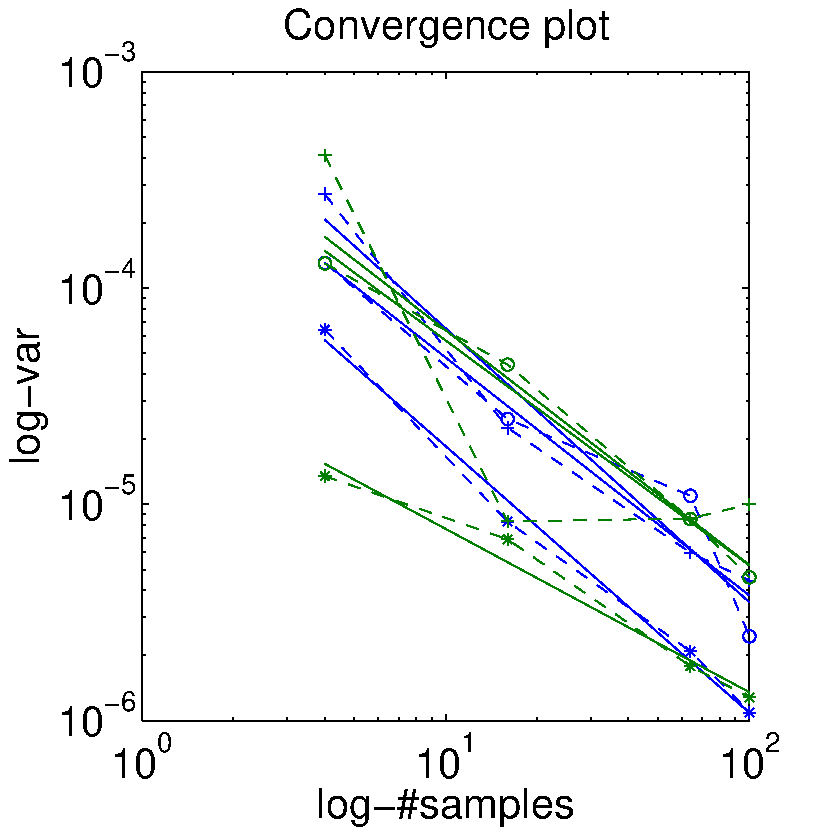
\includegraphics[width=0.36\linewidth]{figs/pbrt-convs.pdf} 
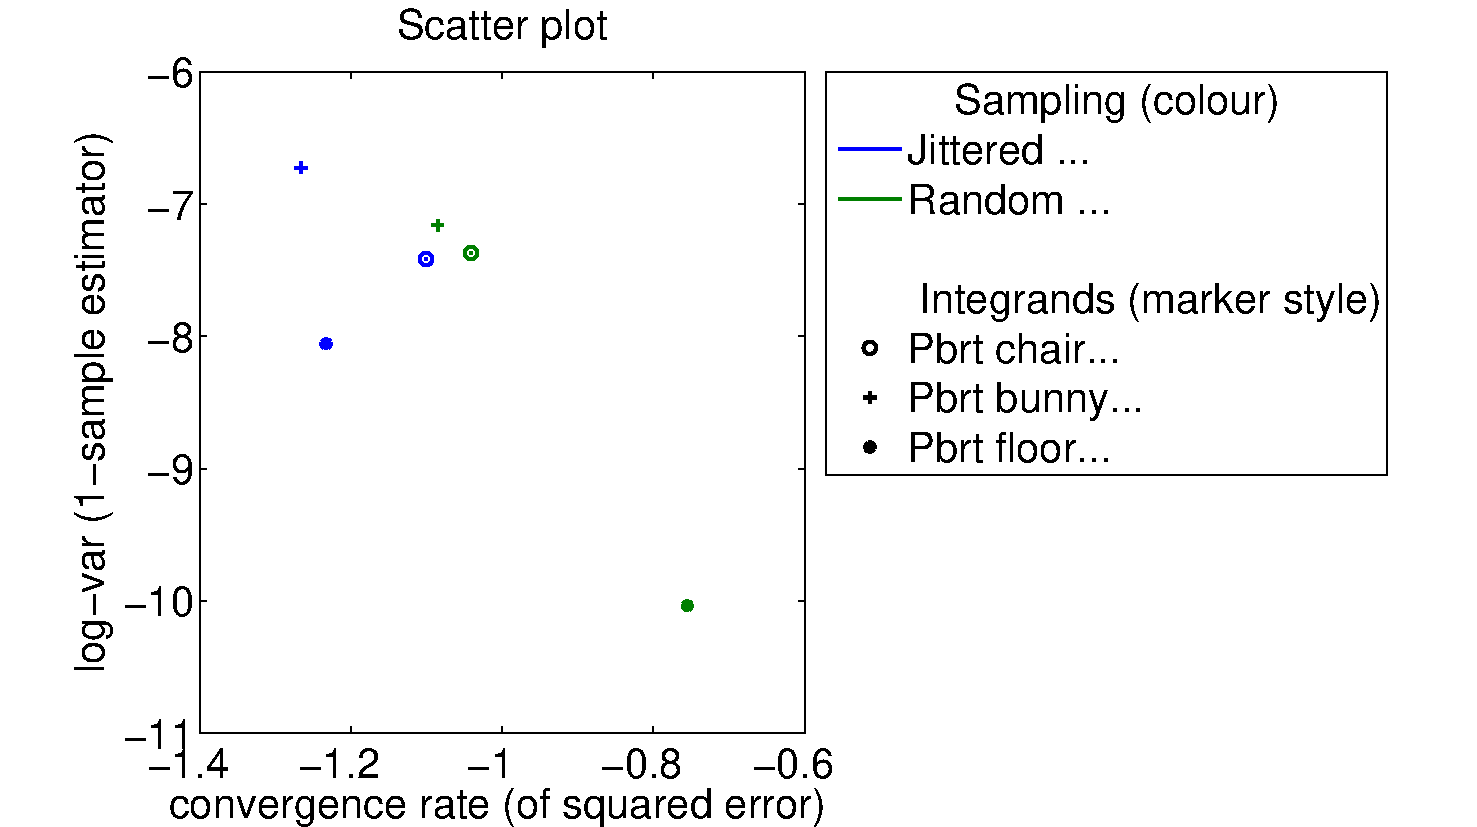
\includegraphics[width=0.64\linewidth]{figs/pbrt-scatter.pdf}
\caption{\label{fig:expbrtint} Example output plots for the code in sec.~\ref{sec:expbrtint}}
\end{figure}

\subsection{Example 2: Comparing other integrands}\label{sec:explotint}
\begin{tcolorbox}
clear; \\
\%  samplers  \\
s(1) = GenSamplStruct('Jittered', '') ; \\
s(2) = GenSamplStruct('Random', '') ; \\
s(3) = GenSamplStruct('BJittered', '--boxwidth .3') ;\\
s(4) = GenSamplStruct('BJittered', '--boxwidth .5') ;\\
s(5) = GenSamplStruct('GJittered', '--sigma .3') ;\\
s(6) = GenSamplStruct('GJittered', '--sigma .5') ;\\
\\
\%  Integrands\\
i(1) = GenIntegStruct('QuadPix', ['--points ' num2str(rand(1,4))]) ;\\
i(2) = GenIntegStruct('PWConstant', '--npts 100 --random') ;\\
% i(3) = GenIntegStruct('Gaussian', '--center .5 .5 --sigma .2 .4') ;\\
i(3) = GenIntegStruct('Disk', '--center .5 .5 --rad .3') ;\\
\\
\\
\% Analysis Parameters\\
ns = [9 36 100 1024 4096] ;\\
nr =  250;\\
ofile = '../out/test';\\
binfile = '../build/eea' ;\\
atype = 'mse' ;\\

system (['rm ' ofile '*.txt']) ;\\
tic\\
data = CollectConvData(ns, nr, ofile, binfile, s, i, atype) ;\\
toc
\end{tcolorbox}

The above matlab code produces two plots (PDF format) with the prefix specified in ofile (see fig.~\ref{fig:explotint}). 
\begin{figure}[htbp]
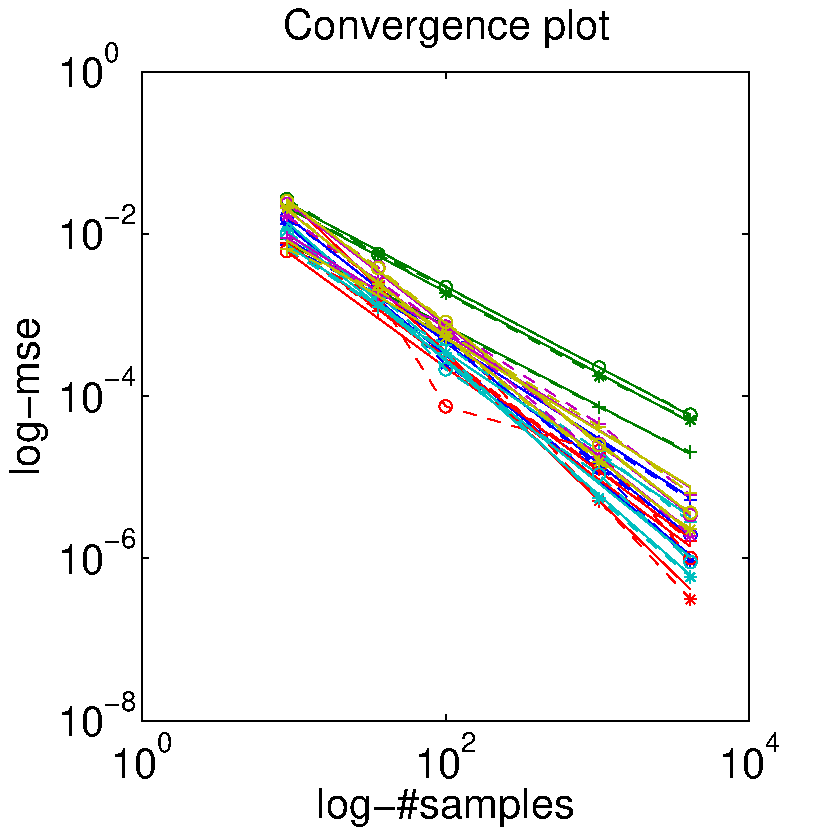
\includegraphics[width=0.36\linewidth]{figs/test-convs.pdf} 
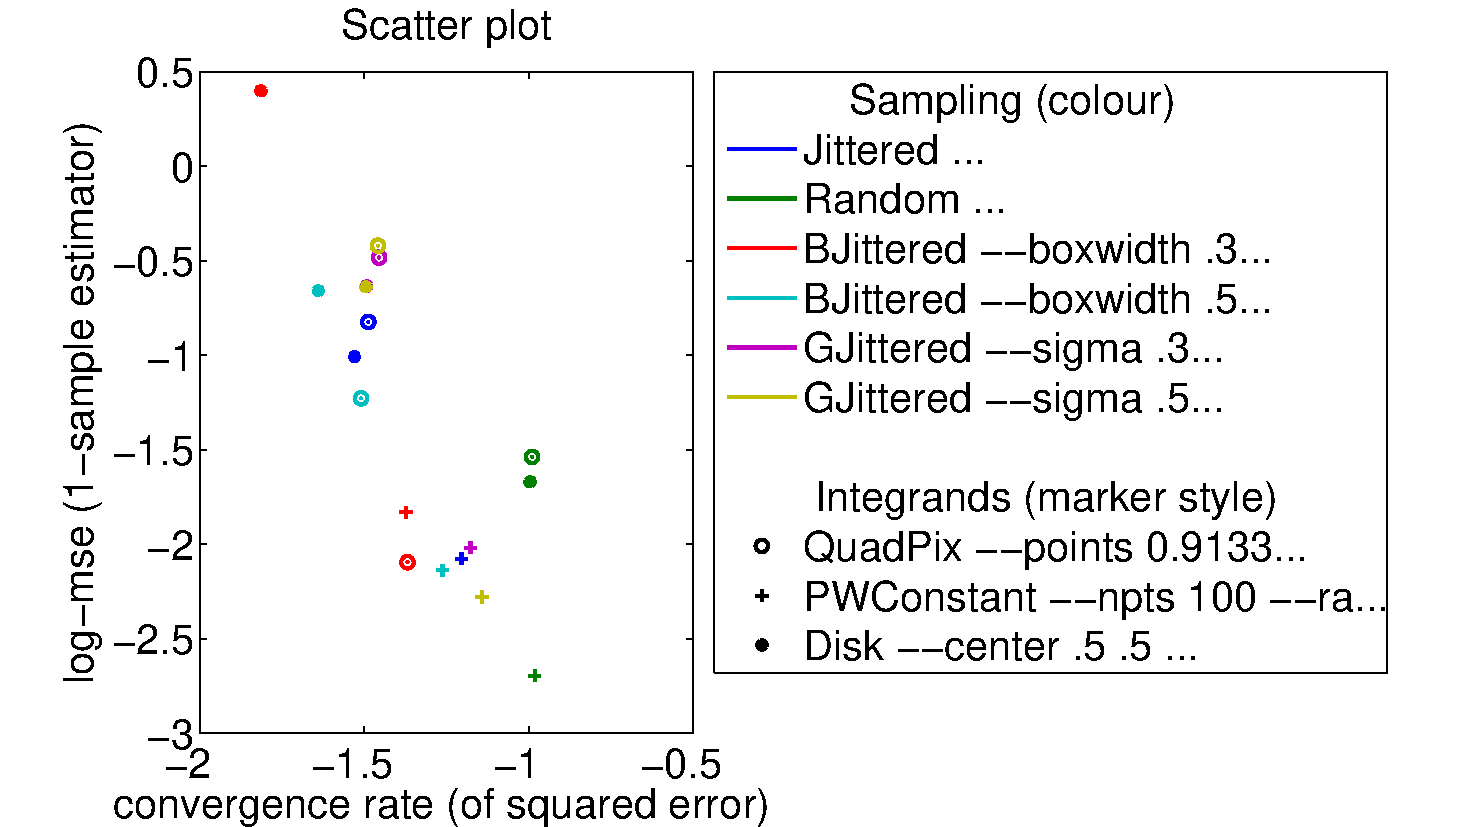
\includegraphics[width=0.64\linewidth]{figs/test-scatter.pdf}
\caption{\label{fig:explotint} Example output plots for the code in sec.~\ref{sec:explotint}}
\end{figure}


\subsection{Example 3: Visualizing point sets}
For visualizing point sets produced by different sampling strategies, no integrand section needs to be specified. The sampling section describes the type of sampling along with any parameters. The analysis section should be set to the type `pts'. The general section should specify the prefix for the output file. 
%
\begin{tcolorbox}
./build/eea \cdash{S} \cdashs{stype} Jittered \cdash{A} \cdashs{atype} pts \cdashs{nsamps} 1024 \cdashs{nreps} 1 \cdash{G} \cdashs{ofile} points
\tcblower
Here, \\
\cdashs{stype}: sampler type (`Jittered'). \\
\cdashs{atype}:  Analyzer type (`pts') \\
\cdashs{nsamps}: Number of samples (`1024') \\
\cdashs{nreps}: Number of trials or realizations (`1') \\
\cdashs{ofile}: Prefix for your output filename (`points')
\end{tcolorbox}

\subsection{Example 4: Visualizing Fourier spectra}
 
 %
Fourier analyzer doesn't need an integrand substring (\cdash{I} $\cdots$). Each analyzer can have different set of subflags (starting with \cdashs). \
For example, the FourierAnalyzer have the following:
%
\begin{tcolorbox}
./build/eea \cdash{S} \cdashs{stype} stratified \cdash{A} \cdashs{atype} fourier \cdashs{nsamps} 4096 \cdashs{nreps} 1 \cdashs{tstep}  2 \cdashs{wstep} 1 \cdash{G} \cdashs{ofile} powerspectrum
\tcblower
Here, \\
\cdashs{stype}: sampler type (stratified, random, etc.). \\
\cdashs{atype}:  Analyzer type (fourier) \\
\cdashs{nsamps}: Number of samples (4096) \\
\cdashs{nreps}: Number of trials or realizations (10) \\
\cdashs{tstep}:  Output intermediate result after given number of trials  \\
\cdashs{wstep}: Frequency step which is 1 for integer frequencies (it can be fractional)\\
\cdashs{ofile}: Prefix for your output filename (could be anything)
\end{tcolorbox}
%


